% !Mode:: "TeX:UTF-8"
%%  本模板推荐以下方式编译:
%%     1. PDFLaTeX[推荐]
%%     2. xelatex [含中文推荐]
%%  注意:
%%  1. 文件默认的编码为 UTF-8 对于windows,请选用支持UTF-8编码的编辑器。
%%   2. 若是模板有什么问题,请及时与我们取得联系,Email:latexstudio@qq.com。
%%   3. 可以到  https://ask.latexstudio.net 提问
%%   4. 请安装 最新版本的 TeXLive 地址:
%%   http://mirrors.ctan.org/systems/texlive/Images/texlive.iso

\documentclass{apmcmthesis}

\usepackage{url}

%%%%%%%%%%%%填写相关信息%%%%%%%%%%%%%%%%%%%%%%%%%%
\tihao{B}                            %选题
\baominghao{apmcm2101137}           %报名号
\begin{document}

\pagestyle{frontmatterstyle}

\begin{abstract}

Thermal photovoltaic technology is a technology that uses various heat sources to heat the heat emitter (absorber), and converts the infrared radiation of the heat emitter into electrical radiation through photovoltaic cells. In order to improve the thermoelectric conversion efficiency of thermal photovoltaic system, the emission spectrum of thermal emitter must be adjusted. The calculation methods of emission spectrum mainly include transfer matrix method (TMM), finite difference time domain method (FDTD) and rigorous coupled wave analysis (RCWA). The main factors affecting the emission spectrum of thermal emitter are the optical properties (refractive index or dielectric constant) and structural properties (thickness). Based on the above theories and three calculation methods, this paper constructs the corresponding model with Origin, Python, SPSS, Microsoft Excel and other software as the working platform.

\keywords{band gap wavelength\quad  thermoelectric conversion efficiency\quad   emission spectrum}
\end{abstract}



\newpage
%目录
\tableofcontents


\newpage
\pagestyle{mainmatterstyle}
\setcounter{page}{1}
\section{Introduction}
\hspace{2em}In order to indicate the origin of problems, the following background is worth mentioning.
\subsection{Background}
\hspace{2em}In recent years, world powers have set their sights on the "star sea" and formulated various space exploration plans. In 2020, China's astronomy 1 will launch and travel through space to Mars; Then in 2021, the rover zhurong completed its expected mission and stayed on Mars. It is still trying to find more discoveries about the vast universe. In order to ensure that various instruments and equipment carried by the rover can operate normally without sunlight and provide necessary technical support for its long-term work, scientists have explored and developed thermal photovoltaic technology. The following figure shows the test prototype of thermal photovoltaic devices. Thermal photovoltaic technology is a technology that uses various heat sources to heat the heat emitter (absorber), and then converts the infrared radiation of the heat emitter into electrical radiation through photovoltaic cells. There are many kinds of heat sources, including chemical energy, solar energy, nuclear energy and so on. The heat emitter in the system mainly uses different material structures to adjust the emission of absorbed heat, so that most of the emitted photons are lower than the band gap wavelength of photovoltaic cells. Photovoltaic cells mainly convert high-energy photons lower than part of the vertical band gap wavelength.\par

\begin{figure}[ht]
\centering
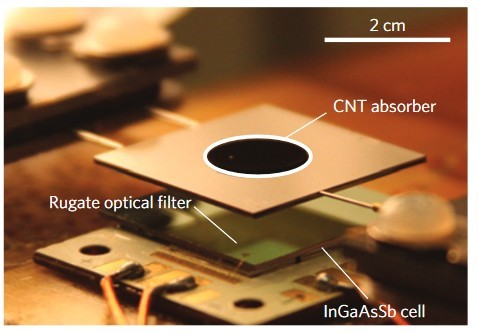
\includegraphics[scale=0.6]{figures/3.jpg}
\caption{The test prototype of the thermophotovoltaic device}
\label{fig:pathdemo}
\end{figure}

\newpage
\section{The Description of the Problem}
\subsection{Problems restatement}
\hspace{2em}The calculation methods of emission spectrum mainly include transfer matrix method (TMM), finite difference time domain method (FDTD) and rigorous coupled wave analysis (RCWA). The main factors affecting the emission spectrum of thermal emitter are the optical properties (refractive index or dielectric constant) and structural properties (thickness). Wang et al. developed a submicron thick multilayer selective solar absorber, which is composed of tungsten, silicon dioxide and silicon nitride, with an absorption rate of up to 0.95 in the solar band. In 2014, Evelyn Wang team of MIT designed a photon controlled solar thermal photovoltaic device, which worked well in the experiment. In their work, the heat emitter is a multilayer thin film structure composed of silicon and silicon dioxide. The thickness of each layer is optimized so that its emission spectrum corresponds to the band gap of antimony indium gallium arsenide (InGaAsSb) battery. Please solve the following problems according to the above description.

\begin{itemize}
  \item Please explain the relationship between the emission spectrum of single-layer structure and material properties (refractive index and thickness), and calculate the emission spectrum of 50 nm thick tungsten within 0.3-5 microns.
  \item Please explain the relationship between the emission spectrum of the multilayer structure and the material properties (refractive index, thickness), and calculate that the emission spectrum (50 nm) of the composite structure formed by tungsten (50 nm) and silica is in the range of 0.3-5 microns.
  \item In order to improve the spectral control ability of the radiator, sometimes the thermal transmitter is designed to emit in the form of narrow band, that is, the emission is concentrated in a very small band, so as to improve the thermoelectric conversion efficiency. Thermal photovoltaic devices, such as the multilayer narrow-band transmitter designed by Sakurai and others with silicon, silicon dioxide and germanium. Please select reasonable materials, design the multi person heat emitter to make its emission as narrow and high as possible, and give the design parameters of multi-layer structure (including the number of layers, material and thickness of each layer) and its emission spectrum. Note that the idea in this problem is that the heat emitter has a sharp and high heat emission at 1.5 microns, and the calculated wavelength range is 0.3-5 microns.
  \item Gallium antimonide (GaSb) batteries are now more advanced. The band gap wavelength is assumed to be 1.71 microns. The emission spectrum of the idealized heat emitter is roughly shown by the red dotted line in the figure below. The blue line represents the external quantum efficiency (EQE), and its influence can be properly considered. Please select reasonable materials, design multilayer heat emitter for GaSb battery to achieve as high thermoelectric conversion efficiency as possible, and give the design parameters of multilayer structure (including number of layers, material and thickness of each layer) and its emission spectrum.

\end{itemize}

\subsection{Problems analysis}
\hspace{2em}These problem mainly involves the analysis of the relationship between band gap wavelength and material properties. The key lies in data mining and processing. Using calculation methods such as transfer matrix method (TMM), finite difference time domain method (FDTD) and strict coupled wave analysis (RCWA), the original data are obtained based on the data provided by accessories and Internet to solve the problem, Then, according to the relevant knowledge required by the discipline and referring to the relevant data, the corresponding mathematical model is established to solve the relevant problems.\par

In view of the problem 1, we should learn the relevant working principle, combined with the corresponding physical knowledge, under the condition of a certain single-layer material and material thickness, find and fit the relationship between wavelength and N, K by controlling variables and using SPSS data analysis software, and get the change law of wavelength by multivariable fitting, so as to solve the problem.\par

In view of the problem 2, we need to calculate the emission spectrum of composite materials. At this time, we need to use the analysis method of control variables. We need to find a reasonable formula through the data in the literature and the Internet, find the relationship between wavelength and N, K, determine the parameters and obtain the emission spectrum.\par

In view of the problem 3, this problem needs to use the Bayesian optimization method to find the objective function and optimization algorithm, and construct the gradient lifting model, so as to gradually obtain the minimum value of the objective function, that is, the optimal solution.\par

In view of the problem 4, this problem is the reverse use of Bayesian formula to achieve the highest possible hot spot conversion efficiency through reasonable parameters. Among them, the parameters can be determined by particle swarm optimization algorithm.\par

\newpage
\section{Models}
\subsection{Basic Model}

\subsubsection{Terms, Definitions and Symbols}
The signs and definitions are mostly generated from queuing theory.
\begin{table}[h!]
  \begin{center}
    \begin{tabular}{c|c} 
      \textbf{Symbol} & \textbf{Meaning}\\
      \hline
      ${\varepsilon_{\bot}}$ & Monochromatic emissivity of an object\\
      ${\rho}$ & Vertical polarization monochromatic emissivity of dielectric to ideal dielectric\\
      a,b & Two auxiliary parameters used in calculation\\
      ${\omega}$ & Inertia factor\\
      ${C_{1},C_{2}}$ & Acceleration constant\\
      random & random number\\
      ${P_{id}}$ & The d-th dimension of the individual extremum of the ith variable\\
      ${P_{gd}}$ & D-Dimension of global optimal solution\\
    \end{tabular}
  \end{center}
\end{table}

\subsubsection{Models and algorithms used}
\begin{itemize}
\item [1)]Bayesian optimization method\par
\qquad Bayesian Optimization establishes an alternative function (probability model) based on the past evaluation results of the objective function to find the value of the minimization objective function. The difference between Bayesian method and random or grid search is that it will refer to the previous evaluation results when trying the next set of super parameters, so it can save a lot of useless work.\par
\qquad The cost of superparametric evaluation is very high, because it requires to use the hyperparametric to be evaluated to train the model once, while many deep learning models can only complete the training and evaluate the model in a few hours and days, so it costs a lot. Bayesian parameter tuning uses a constantly updated probability model to "focus" promising hyperparameters by inferring past results.\par

\item [2)]Selection in Python\par
\qquad There are several Bayesian Optimization libraries in Python, and their alternative functions of objective functions are different. In this article, we will use hyperopt, which uses tree Parzen estimator (TPE) and other Python libraries, including spearint (Gaussian process proxy) and Smac (random forest regression)\par

\item [3)]Four parts of optimization problem\par
\begin{itemize}
\item Objective function: we want to minimize the content. Here, the objective function is the loss of the machine learning model on the verification set using this set of super parameters.
\item Domain space: the value range of the super parameter to search
\item Optimization algorithm: a method of constructing an alternative function and selecting the next hyperparametric value for evaluation.
\item Result history: stored results from objective function evaluation, including hyperparameters and losses on validation sets
\end{itemize}
\item [3)]Data set\par
\qquad In this example, we will use the caravan insurance dataset, whose goal is to predict whether a customer will purchase an insurance policy. This is a supervised classification problem. The size of training set and test set are 5800 and 4000 respectively. The indicators for evaluating performance are AUC (area under the curve) evaluation criteria and ROC (receiver operating characteristic) curve. The higher the rocauc, the better the model.\par
\qquad To minimize the objective function for hyperopti, our objective function returns 1-rocauc, thereby improving ROC auco.
\item [4)]Gradient lifting model\par
\qquad Gradient elevator (GBM) is a model based on combining weak learners (such as decision tree) into strong learners. There are many hyperparameters in GBM to control the whole set and a single decision tree, such as the number and depth of decision trees. After a brief understanding of GBM, we introduce the four parts of the optimization model corresponding to this problem

\end{itemize}

\subsubsection{Solution and Result}
\begin{itemize}
\item [1)]In view of the problem 1, in fact, OES is an analytical technology for detecting various metal components, which is widely used and trusted. AES, also known as atomic emission spectrometry, is widely used in reality.\par

\qquad OES technology can detect metal melt, metal semi-finished products / finished products, metal processing industry, pipes, bolts, bars, wires, plates, etc.\par

\qquad The electromagnetic spectrum used by oes includes visible spectrum and partial ultraviolet spectrum. The wavelength range is 130nm to about 800 nm.\par

\qquad OES can analyze various elements from lithium to uranium in solid metals, and has the advantages of high accuracy and precision and low detection limit.\par

\qquad Emission spectrometers are composed of three parts: light source, which can excite atoms in metal samples to emit characteristic spectra.\par

\qquad The second part is the optical system. The composite emission spectrum emitted when the sample evaporates is called plasma and enters the spectrometer. The diffraction grating in the spectrometer will disperse the incoming spectrum according to the wavelength, and then measure the spectral line intensity of each wavelength through the corresponding detector. The measured spectral line intensity is directly proportional to the element concentration in the sample.\par

\qquad The third part is computer system. After the computer system obtains the measured strength, it will process the data through the preset calibration program and obtain the element concentration. The user interface can directly and clearly display the processing results, requiring only a small amount of operation by the operator, and the results can also be printed or saved for future use.\par

\qquad When the energy of discharge interacts with metal atoms, some electrons in the outer layer of atoms will transition. Because the outer electron is far from the nucleus and the adsorption force is weak, the energy required for its transition is also less. Holes are formed after electron transition, which makes the atom unstable.\par

\begin{figure}[ht]
\centering
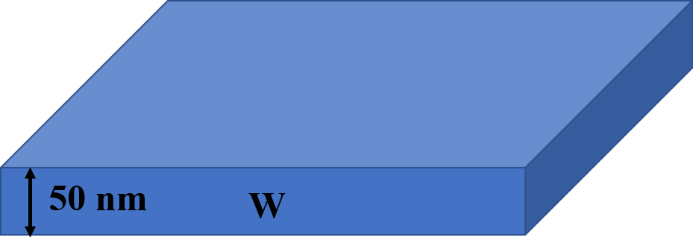
\includegraphics[scale=0.5]{figures/4.png}
\caption{The schematic of 50-nanometer-thick tungsten}
\label{fig:pathdemo}
\end{figure}


\qquad In order to restore stability, high orbit electrons far from the nucleus will fall back to fill the holes. The excess energy released by electrons moving between two energy levels will be emitted in the form of element characteristic spectral lines.\par

\qquad The detector will collect the peak signal of each spectral line, generate a spectrum after processing, and display the light intensity and corresponding wavelength. This means that oes can conduct qualitative analysis / quantitative analysis.\par

\qquad The peak wavelength can be used to determine the element type, and the peak area or intensity can show the content of the element in the sample.\par

\qquad OES has many advantages: low cost, fast speed, simple operation, capable of measuring a wide range of elements, including carbon, sulfur, phosphorus, boron, nitrogen and other important elements. It has high accuracy in measuring trace and impurity elements.\par

\qquad OES is the first choice for trace metal analysis. At present, it is also the only method that can be used for on-site analysis of carbon and nitrogen outside the laboratory.\par

\qquad However, in the final analysis, due to the uncertainty of wavelength, the detection of tungsten needs to have a certain inspection standard for OES, which is the current standard of emission spectrometric analysis of tungsten of the people's Republic of China.\par

\qquad Emission spectrometric analysis method of tungsten (YS / t559-2009) specifies the determination method of iron, silicon, aluminum, manganese, magnesium, nickel, titanium, vanadium, cobalt, cadmium, arsenic, lead, bismuth, tin, antimony, copper, chromium, calcium and molybdenum in tungsten and tungsten compounds. It is applicable to the determination of iron, silicon, aluminum, manganese, magnesium, nickel, titanium, vanadium, cobalt, cadmium, arsenic, lead, bismuth, tin, antimony, copper, chromium, calcium and molybdenum in tungsten and tungsten compounds. Emission spectrum analysis method of tungsten (YS / T 559-2009) was drafted by Chongyi Zhangyuan Tungsten Products Co., Ltd. and Luoyang Luanchuan molybdenum industry group. Main drafters: Tan Taizhang, Wang Pei, Wei Li.
\qquad On the third page, we can find the wavelength data and the intensity values corresponding to different wavelengths (these quantities can be used to draw the spectrum).\par

It can be seen from the table that the required wavelength is about 330nm.\par

\begin{figure}[ht]
\centering
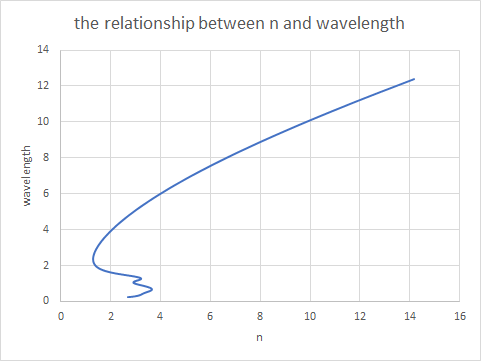
\includegraphics[scale=0.5]{figures/1.png}
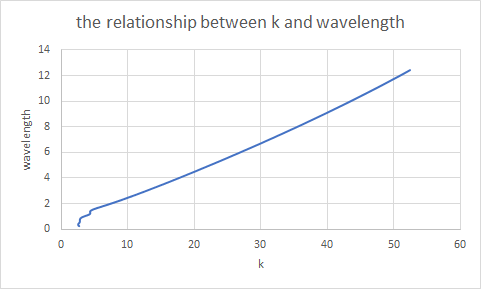
\includegraphics[scale=0.6]{figures/2.png}
\caption{The relationship between wavelength and N and K, respectively}
\label{fig:pathdemo}
\end{figure}

\item [2)]In view of the problem b, because the spectrum is still electromagnetic wave in the final analysis, electromagnetic theory can be used to explain the characteristics of thermal radiation propagation of composites. According to the electromagnetic theory analysis of the object surface, the thermal emissivity of the actual object surface, i.e. emissivity and absorptivity, mainly depends on the optical constant. Therefore, the monochromatic emissivity of the object can be expressed by the following formula:\par
\[\varepsilon_{\bot}(\theta)=\frac{1}{2}\{{[1-\rho_{A,\bot}]+[1-\rho_{A,\square}]}\}=\]\par
\[\frac{2acos\theta}{a^2+b^2+2abcos\theta+cos^2\theta}\bullet\]\par
\[1+\frac{a^2+b^2+sin^2\theta}{cos^2\theta(a^2+b^2+2asin\theta tan\theta+sin^2\theta tan\theta)}\]\par
among $\rho$ is the vertical polarization oriented monochromatic emissivity of general medium to ideal dielectric. The relationship between parameters a and b can be solved by the following formula:\par
\[2a^2=\sqrt{(n^2-k^2-sin^2\theta)^2+4n^2 k^2}+(n^2-k^2-sin^2\theta)\]\par
\[2b^2=\sqrt{(n^2-k^2-sin^2\theta)^2+4n^2 k^2}-(n^2-k^2-sin^2\theta)\]\par
\qquad The normal spectral emissivity is the spectrum. As long as it is not absolute zero, any object can radiate infrared electromagnetic wave. The indicators of far-infrared radiation energy of matter include radiation power and radiance, but emissivity is often used to characterize in practical application. \qquad Emissivity refers to the ratio of the radiation power (or radiance) of the test sample to the radiation power (or radiance) of the blackbody at a certain temperature within a wavelength interval. Emissivity is a positive number between 0 and 1. Generally, emissivity depends on material properties, environmental factors and observation conditions\par
\qquad As can be seen from the figure, there is a maximum value for the spectral emissivity of different objects with the change of monochromatic refractive index. On the left side of the maximum value, the emissivity increases with the refractive index. From the above analysis, it can be seen that the monochromatic absorption index and monochromatic refractive index of the object decrease, and the normal spectral emissivity increases.\par
\qquad According to the thermal radiation medium absorption model, the relationship between radiation intensity and material can be obtained:\par
\[I(x,\nu)=I_{0}(v)exp[-\alpha(v)x]\]\par

\begin{figure}[ht]
\centering
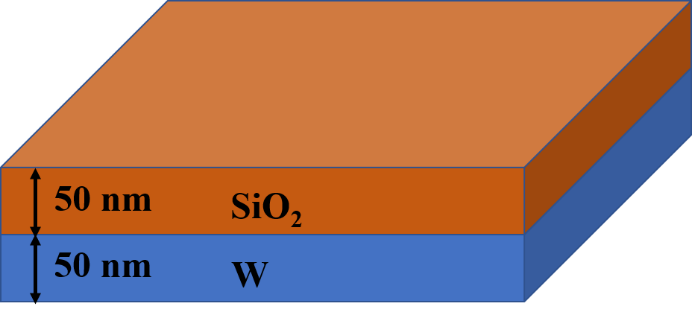
\includegraphics[scale=0.3]{figures/5.png}
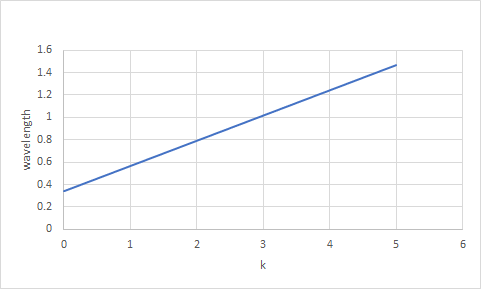
\includegraphics[scale=0.6]{figures/6.png}
\caption{The schematic of multilayer structure formed by tungsten and silica}
\label{fig:pathdemo}
\end{figure}

\quad A simple equation was obtained by multivariate linear fitting using SPSS
\[wavelength=0.006n+0.226k+0.036\]\par

\qquad According to the spectral standards of tungsten and silicon dioxide involved in the previous industrial standards of the people's Republic of China for tungsten, it can be obtained that the wavelength of tungsten is recorded as X, which is 330nm, and the wavelength of silicon dioxide is recorded as V, which is about 450nm. Through the above formula, the emission spectrum can be calculated to be about 417nm.\par

\item [3)]In this problem, we want to use Bayesian algorithm and its optimization algorithm, including objective function, domain space, optimization algorithm and result history. At the same time, the data set is used to find the minimized objective function and determine the parameters, so as to obtain the best structural parameters, and find the most suitable material according to the data table provided.\par
The model used has been mentioned in the previous part, and the specific code implementation is put in the last part of the article.\par

\item [4)]This problem uses particle swarm optimization algorithm, which is implemented in the code at the end of the paper
The algorithm flow is as follows:\par
\begin{itemize}
\item 1. Initialization\par
Firstly, we set the maximum number of iterations, the number of independent variables of the objective function, the maximum speed of particles and the position information as the whole search space. We randomly initialize the speed and position in the speed interval and search space, set the particle swarm size to m, and each particle randomly initializes a flying speed.
\item 2. Individual extremum and global optimal solution\par
The fitness function is defined. The individual extremum is the optimal solution found for each particle. Finding a global value from these optimal solutions is called this global optimal solution. Compare with the historical global optimum and update it.
\item 3. Update formulas for speed and position
\[V_{m}=\omega V_{id}+c_{1}random(0,1)(P_{id}-X_{id})+C_{2}random(0,1)(P_{gd}-X_{id})\]
\[X_{id}=X_{id}+V_{id}\]\par
\item 4.Termination conditions\par
\begin{itemize}
\item Set number of iterations reached
\item The difference between algebras satisfies the minimum limit

\begin{figure}[ht]
\centering
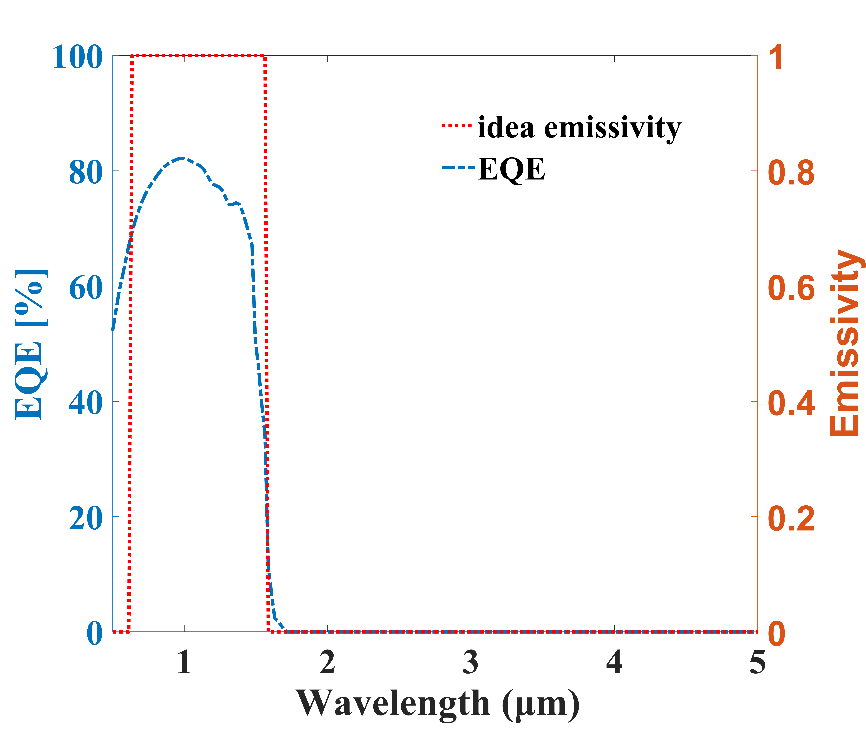
\includegraphics[scale=0.3]{figures/7.png}

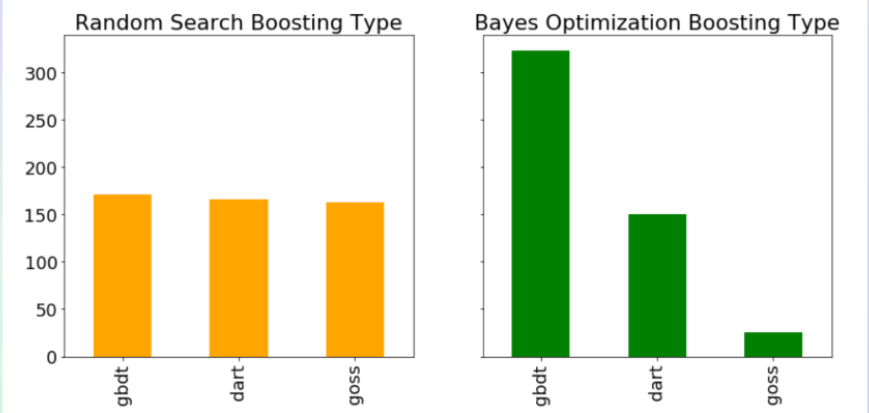
\includegraphics[scale=0.4]{figures/8.png}
\caption{The EQE and ideal emission spectrum of GaSb for thermophotovoltaic}
\label{fig:pathdemo}
\end{figure}

\end{itemize}
\end{itemize}
\end{itemize}

\newpage
\section{Conclusions}
\subsection{Conclusions of the problem}
\begin{itemize}
\item In the problem 1, we learned the relevant working principle, combined with the corresponding physical knowledge, under the condition of a certain single-layer material and material thickness, find and fit the relationship between wavelength and N, K by controlling variables and using SPSS data analysis software, and get the change law of wavelength by multivariable fitting, so as to solve the problem.
\item In the problem 2, we need to calculate the emission spectrum of composite materials. At this time, we need to use the analysis method of control variables. We need to find a reasonable formula through the data in the literature and the Internet, find the relationship between wavelength and N, K, determine the parameters and obtain the emission spectrum.
\item In the problem 3, this problem needs to use the Bayesian optimization method to find the objective function and optimization algorithm, and construct the gradient lifting model, so as to gradually obtain the minimum value of the objective function, that is, the optimal solution.
\item In the problem 4, this problem is the reverse use of Bayesian formula to achieve the highest possible hot spot conversion efficiency through reasonable parameters. Among them, the parameters can be determined by particle swarm optimization algorithm.
\end{itemize}	
\subsection{Methods used in our models}
\begin{itemize}
\item Bayesian optimization method
\item Selection in Python
\item Four parts of optimization problem
\begin{itemize}
\item Objective function
\item Domain space
\item Optimization algorithm
\item Result history
\end{itemize}
\end{itemize}

%参考文献
\newpage
\begin{thebibliography}{9}%宽度9
\bibitem{1} Lee G J; Lee Y, Jung S G, Jung B Y, Hwangbo C K, Kim S, Park I 2007 Design, fabrication, linear and nonlinear optical properties of metal-dielectric photonic bandgap structures Journal of Korean Physical Society 51 431, 2007.
\bibitem{2} Carrera-Escobedo V, Rosu H 2016 Electromagnetic transmittance in alternating materialmetamaterial layered structures. arXiv preprint arXiv:1610.0021., 2016.
\bibitem{3} Born M, Wolf E 2013 Principles of optics: electromagnetic theory of propagation, interference and diffraction of light. Elsevier., 2013.
\bibitem{4} J. Pawlikovski, “Comments on the determination of the absorption coefficient of thin semiconductor films,” Thin Solid Films 127, 29–38 1985.
\bibitem{5} C. J. Gabriel and A. Nedoluha, “Transmittance and reflectance of systems of thin and thick layers,” Opt. Acta 18, 415–423, 1971.
\bibitem{6} N. Hatzopoulos, W. Skorupa, and D. Siapkas, “Double Simox structures formed by sequential high energy oxygen implantation into silicon,” J. Electrochem. Soc. 147, 354–362 2000. 32. D. I. Siapkas, D. B. Kushev, N. N. Zheleva, J. Siapkas, and I. Lelidis, “Optical constants of tin-telluride determined from infrared interference spectra,” Infrared Phys. 31, 425–433, 1991.
\bibitem{7} V. Stelmakh, V. Rinnerbauer, R. Geil, P. Aimone, J. Senkevich, J. Joannopoulos, M. Soljačić, I. Celanovic, High-temperature tantalum tungsten alloy photonic crystals: stability, optical Properties, and fabrication, Appl. Phys. Lett. 103 (2013) 123903.
\bibitem{8} Wang, C. A. et al. High-quantum-efficiency 0.5 eV GaInAsSb/GaSb thermophotovoltaic devices. Appl. Phys. Lett. 75, 1305–1307 (1999).
\bibitem{9} Yamawaki, M.; Ohnishi, M.; Ju, S.; Shiomi, J. Multifunctional structural design of graphene thermoelectrics by Bayesian optimization. Sci. Adv. 2018, 4 (6), No. eaar4192.
\end{thebibliography}

\newpage
%附录

\section{Appendix}
\begin{lstlisting}[language=python,caption={the python objective function definition}]
def objective(hyperparameters):
    '''Returns validation score from hyperparameters'''
     model = Classifier(hyperparameters)
    validation_loss = cross_validation(model, training_data)
    return validation_loss

 \end{lstlisting}
\begin{lstlisting}[language=python,caption={Use 10\% off cross validation and early stop}]
import lightgbm as lgb
from hyperopt import STATUS_OK
N_FOLDS = 10
# Create the dataset
train_set = lgb.Dataset(train_features, train_labels)
def objective(params, n_folds=N_FOLDS):
   '''Objective function for Gradient Boosting Machine Hyperparameter Tuning'''
   # Perform n_fold cross validation with hyperparameters
   # Use early stopping and evalute based on ROC AUC
   cv_results = lgb.cv(params, train_set, nfold=n_folds, num_boost_round=10000,
                       early_stopping_rounds=100, metrics='auc', seed=50)
   # Extract the best score
   best_score = max(cv_results['auc-mean'])
   # Loss must be minimized
   loss = 1 - best_score
   # Dictionary with information for evaluation
   return {'loss': loss, 'params': params, 'status': STATUS_OK}
 \end{lstlisting}
\begin{lstlisting}[language=python,caption={All superparameters in GBM}]
import lgb
# Default gradient boosting machine classifier
model = lgb.LGBMClassifier()
model
LGBMClassifier(boosting_type='gbdt', n_estimators=100,
              class_weight=None, colsample_bytree=1.0,
              learning_rate=0.1, max_depth=-1,
              min_child_samples=20,
              min_child_weight=0.001, min_split_gain=0.0,
              n_jobs=-1, num_leaves=31, objective=None,
              random_state=None, reg_alpha=0.0, reg_lambda=0.0,
              silent=True, subsample=1.0,
              subsample_for_bin=200000, subsample_freq=1)
 \end{lstlisting}
\begin{lstlisting}[language=python,caption={Definition of domain}]
# Define the search space
space = {
   'class_weight': hp.choice('class_weight', [None, 'balanced']),
   'boosting_type': hp.choice('boosting_type',
                              [{'boosting_type': 'gbdt',
                                   'subsample': hp.uniform('gdbt_subsample', 0.5, 1)},
                                {'boosting_type': 'dart',
                                    'subsample': hp.uniform('dart_subsample', 0.5, 1)},
                                {'boosting_type': 'goss'}]),
'num_leaves': hp.quniform('num_leaves', 30, 150, 1),
   'learning_rate': hp.loguniform('learning_rate', np.log(0.01), np.log(0.2)),
   'subsample_for_bin': hp.quniform('subsample_for_bin', 20000, 300000, 20000),
   'min_child_samples': hp.quniform('min_child_samples', 20, 500, 5),
   'reg_alpha': hp.uniform('reg_alpha', 0.0, 1.0),
   'reg_lambda': hp.uniform('reg_lambda', 0.0, 1.0),
   'colsample_bytree': hp.uniform('colsample_by_tree', 0.6, 1.0)
}
 \end{lstlisting}
\begin{lstlisting}[language=python,caption={Sample from the full space}]
# Sample from the full space
example = sample(space)

# Dictionary get method with default
subsample = example['boosting_type'].get('subsample', 1.0)

# Assign top-level keys
example['boosting_type'] = example['boosting_type']['boosting_type']
example['subsample'] = subsample
example
{'boosting_type': 'gbdt',
'class_weight': 'balanced',
'colsample_bytree': 0.8111305579351727,
'learning_rate': 0.16186471096789776,
'min_child_samples': 470.0,
'num_leaves': 88.0,
'reg_alpha': 0.6338327001528129,
'reg_lambda': 0.8554826167886239,
'subsample_for_bin': 280000.0,
'subsample': 0.6318665053932255}
 \end{lstlisting}
\begin{lstlisting}[language=python,caption={Return result of super parameter}]
{'boosting_type': 'gbdt',
  'class_weight': 'balanced',
  'colsample_bytree': 0.7125187075392453,
  'learning_rate': 0.022592570862044956,
  'min_child_samples': 250,
  'num_leaves': 49,
  'reg_alpha': 0.2035211643104735,
  'reg_lambda': 0.6455131715928091,
  'subsample': 0.983566228071919,
  'subsample_for_bin': 200000}
 \end{lstlisting}

\begin{lstlisting}[language=matlab,caption={PSO algorithm}]
clc
clear 
close all
E=0.000001; 
maxnum=800;% Maximum number of iterations
narvs=2;% Number of independent variables of objective function
particlesize=50;% Particle swarm size
c1=2;% Individual learning factor of each particle, acceleration constant
c2=2;% Social learning factor of each particle, acceleration constant
w=0.6;% Inertia factor
vmax=5;% Maximum flying speed of particles
v=2*rand(particlesize,narvs);% Particle flying speed
x=-300+600*rand(particlesize,narvs);% Particle location
% Define fitness function
fitness=inline('(x(1)^2+x(2)^2)/10000','x');
for i=1:particlesize
	f(i)=fitness(x(i,:));	
end
personalbest_x=x;
personalbest_faval=f;
[globalbest_faval,i]=min(personalbest_faval);
globalbest_x=personalbest_x(i,:); 
k=1;
while (k<=maxnum)
	for i=1:particlesize
			f(i)=fitness(x(i,:));
		if f(i)<personalbest_faval(i)
			personalbest_faval(i)=f(i);
			personalbest_x(i,:)=x(i,:);
		end
	end
[globalbest_faval,i]=min(personalbest_faval);
	globalbest_x=personalbest_x(i,:);
	for i=1:particlesize
		v(i,:)=w*v(i,:)+c1*rand*(personalbest_x(i,:)-x(i,:))...
			+c2*rand*(globalbest_x-x(i,:));
		for j=1:narvs
			if v(i,j)>vmax
				v(i,j)=vmax;
			elseif v(i,j)<-vmax
				v(i,j)=-vmax;
            end
		end
		x(i,:)=x(i,:)+v(i,:);
 
    end
    ff(k)=globalbest_faval;
    if globalbest_faval<E
        break
    end
%       figure(1)
%       for i= 1:particlesize
%       plot(x(i,1),x(i,2),'*')
%       end
	k=k+1;
end
xbest=globalbest_x;
figure(2)
set(gcf,'color','white');
plot(1:length(ff),ff)

 \end{lstlisting}

\end{document} 